\documentclass[12pt,a4paper]{article}
%\usepackage{epsf,epic,eepic,eepicemu}
%\documentstyle[epsf,epic,eepic,eepicemu]{article}

\usepackage[pdftex]{graphicx}
\usepackage[utf8]{inputenc} %kodovani znaku v textovem souboru
%\usepackage[T1]{fontenc} %kodovani znaku na vystupu
\usepackage[czech]{babel} %prizpusobeni jazyku, napr. deleni slov
%\usepackage{a4wide}

\begin{document}
\title{Semestrální projekt MI-PAP, MI-PRC 2014/2015\\
Násobení matic \\
\vspace{10px}}
\author{Karel Fiala \\
\vspace{10px} \\
\small České vysoké učení technické v~Praze\\
\small Fakulta informačních technologií\\
\small Thákurova 9, 160 00 Praha 6\\
\small Česká republika \\
\vspace{10px} \\
}
\date{\today}
\maketitle

%\oddsidemargin=-5mm \evensidemargin=-5mm \marginparwidth=.08in
%\marginparsep=.01in \marginparpush=5pt \topmargin=-15mm
%\headheight=12pt \headsep=25pt \footheight=12pt \footskip=30pt
%\textheight=25cm \textwidth=17cm \columnsep=2mm \columnseprule=1pt
%\parindent=15pt\parskip=2pt

% ===== ZADANI =====

%Kapitola 1
%- Definici problému
%- Popis sekvenčního algoritmu a jeho implementace
%
%Kapitola 2 (pro OpenMP)
%- Popis případných úprav algoritmu a jeho implementace, včetně volby datových struktur
%- Zda byla využita vektorizace (popř. proč jí nemožno využít)
%- Popis optimalizací pro dosažení lineárního zrychlení
%- Tabulkově a případně graficky zpracované naměřené hodnoty časové složitosti měřených instancí běhu (optimalizované implementace) programu s popisem instancí dat
%- Analýza a hodnocení vlastností dané implementace programu.
%
%Kapitola 4 (pro CUDA)
%- Popis případných úprav algoritmu a jeho implementace, včetně volby datových struktur
%- Popis optimalizací pro dosažení efektivní implementace
%- Tabulkově a případně graficky zpracované naměřené hodnoty časové složitosti měřených instancí běhu (optimalizované implementace) programu s popisem instancí dat
%- Analýza a hodnocení vlastností dané implementace programu.
%
%Kapitola 5
%- Závěr (včetně porovnání výkonnosti všech tří verzí)
%- (případně) Literatura

\clearpage
\tableofcontents
\clearpage

\section{Definice problému a popis sekvenčního algoritmu}
\subsection{Definice problému}

Násobení matic pomocí klasického algoritmu a rekurzivního Strassenova algoritmu.

\subsection{Popis sekvenčního algoritmu a jeho implementace}

\subsubsection{Klasický multiplikační algoritmus}
Násobíme matici $B$ maticí $A$ tak, že výsledný prvek matice $C$ je součtem součinů čísel v~řádku matice $A$ s~příslušným číslem ve sloupci matici $B$.

\bigskip
Výpočetní náročnost klasického algoritmu je $O(n^3)$.

\bigskip
Klasický multiplikační algoritmus je implementován třemi vnořenými cykly, kde první dva určují řádek a sloupec výsledné matice a třetí tvoří součet součinů prvků násobených matic.

\bigskip
Algoritmus je časově i paměťové stabilní.

\subsubsection{Strassenův rekurzivní algoritmus}

Strassenův rekurzivní algoritmus je asymptoticky rychlejší než klasický multiplikační algoritmus. Využívá pouze 7 násobení místo 8 jako je tomu u~klasického multiplikačního algoritmu.

\bigskip
Strassenův rekurzivní algoritmus pracuje se složitostí $O(n^{\log_2{7}}) \approx O(n^{2.807})$. 

\bigskip
V~mé implementaci se pro matice řádu 500 a nižší použije klasický multiplikační algoritmus, který je efektivnější.


\section{OpenMP}
\subsection{Popis implementace}

\subsubsection{Klasický multiplikační algoritmus}

V~podstatě bez úprav.

\bigskip
Paralelizace spočívá ve vložení následujícího řádku před první cyklus.

\begin{verbatim}
#pragma omp parallel for shared(C) private(i) schedule(dynamic,10)
\end{verbatim}

\bigskip
Dělení práce po 10ti \uv{kusech} snižuje režii v~případě velkých vstupních matic. Jeden řádek matice je zpracován velmi rychle.


\subsubsection{Strassenův rekurzivní algoritmus}

Úprav v~celém programu je opět minimálně.
\bigskip

Místo přímého volání Strassenova rekurzivního algoritmu je zavolán \uv{wrapper}, který se postará o~rozdělení dvou vstupních matic na $2*16$ podmatic. Jednotlivá vlákna poté volají Strassenův rekurzivní algoritmus na násobení dvou menších matic. Těchto volání je 64, protože každý prvek výsledné matice je složen ze 4 součinů podmatic.
\bigskip

Takto implementovaný algoritmus tedy dokáže využít maximálně 64 procesorových jader.

\bigskip
64 podmatic je poté paralelně redukováno na 32 podmatic a poté opět paralelně redukováno na 16 výsledných podmatic. Tyto matice jsou již částmi chtěného výsledku.


\subsection{Použití vektorizace}

\subsubsection{Klasický multiplikativní algoritmus}

\begin{verbatim}
src/simd_trivial.cpp:7: note: vectorized 0 loops in function.
src/main.cpp:17: note: vectorized 0 loops in function.
src/main.cpp:33: note: vectorized 0 loops in function.
src/main.cpp:50: note: vectorized 0 loops in function.
src/main.cpp:78: note: vectorized 0 loops in function.
src/main.cpp:103: note: vectorized 0 loops in function.
src/main.cpp:149: note: vectorized 0 loops in function.
\end{verbatim}


\subsubsection{Strassenův rekurzivní algoritmus}

\begin{verbatim}
src/simd_strassen.cpp:353: note: vectorized 1 loops in function.
src/simd_strassen.cpp:347: note: vectorized 1 loops in function.
src/simd_strassen.cpp:367: note: vectorized 4 loops in function.
src/main.cpp:17: note: vectorized 0 loops in function.
src/main.cpp:33: note: vectorized 0 loops in function.
src/main.cpp:50: note: vectorized 0 loops in function.
src/simd_strassen.cpp:8: note: vectorized 0 loops in function.
src/simd_strassen.cpp:13: note: vectorized 0 loops in function.
src/simd_strassen.cpp:29: note: vectorized 1 loops in function.
src/simd_strassen.cpp:41: note: vectorized 1 loops in function.
src/simd_strassen.cpp:53: note: vectorized 1 loops in function.
src/simd_strassen.cpp:68: note: vectorized 1 loops in function.
src/simd_strassen.cpp:80: note: vectorized 0 loops in function.
src/simd_strassen.cpp:90: note: vectorized 30 loops in function.
src/simd_strassen.cpp:330: note: vectorized 0 loops in function.
src/simd_strassen.cpp:191: note: vectorized 12 loops in function.
src/main.cpp:78: note: vectorized 0 loops in function.
src/main.cpp:103: note: vectorized 0 loops in function.
src/main.cpp:149: note: vectorized 0 loops in function.
src/main.cpp:171: note: vectorized 0 loops in function.

\end{verbatim}



\subsection{Popis optimalizací pro dosažení lineárního zrychlení}

Vše bylo kompilováno s~parametrem $-O3$.

\subsubsection{Klasický multiplikační algoritmus}

Žádné speciální optimalizace.


\subsubsection{Strassenův rekurzivní algoritmus}

Snaha o~zmenšení režie při práci s~podmaticemi, např. pomocí paralelizace redukce.




\pagebreak
\subsection{Naměřené výsledky}


\subsubsection{Klasický multiplikační algoritmus}


\begin{center}
\begin{tabular}{ | c || c | c | c | c | }
\hline
\#CPU    &   1000		&	2000	&	3000	&	4000	\\
\hline
\hline
1    &   11.365326		&	103.732902	&	264.885942 	& 450.300757 	\\ \hline
2    &   5.683157		&	25.049751	&	197.348525 	& 314.536432 	\\ \hline
4    &   2.847626		&	25.096038	&	99.390237 	& 180.675981 	 \\	 \hline
8    &   1.486099		&	12.946192	&	49.909194 	& 108.842585	\\	 \hline
12   &   1.034171		&	8.721059 	&	32.952173	& 90.281103 	\\	 \hline
24   &   1.031660		&	9.081376	&	34.469956	& 89.329224  	\\ \hline
\end{tabular}
\end{center}

\pagebreak
\begin{figure}[h]
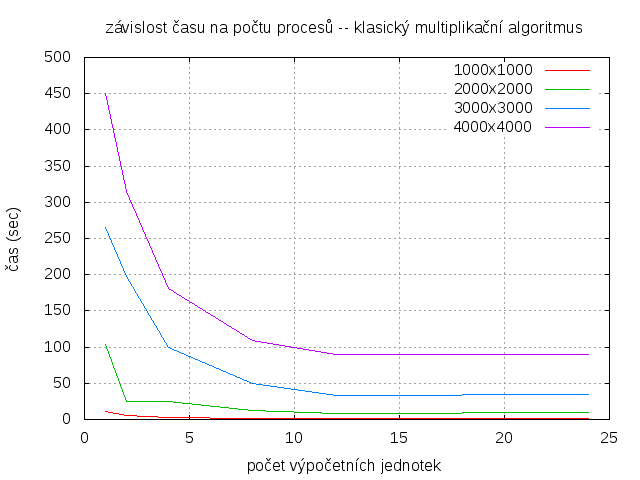
\includegraphics[width=\textwidth]{graph/classic.png}
\caption{Klasický multiplikační algoritmus}
\label{data4}
\end{figure}

\pagebreak
\begin{figure}[h]
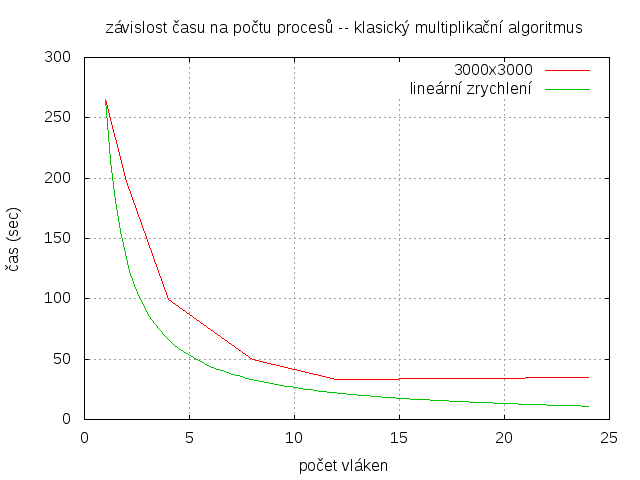
\includegraphics[width=\textwidth]{graph/classic-3000.png}
\caption{Klasický multiplikační algoritmus pro matici 3000x3000}
\label{data4}
\end{figure}

\pagebreak
\begin{figure}[h]
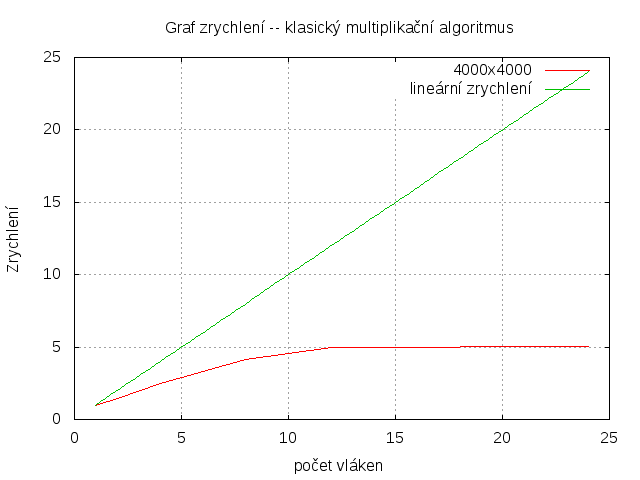
\includegraphics[width=\textwidth]{graph/classic-acc.png}
\caption{Graf zrychlení klasického multiplikačního algoritmu pro matici 4000x4000}
\label{data4}
\end{figure}



\pagebreak
\subsubsection{Strassenův rekurzivní algoritmus}


\begin{center}
\begin{tabular}{ | c || c | c | c | c | }
\hline
\#CPU    &   1000		&	2000	&	3000	&	4000	\\
\hline
\hline
1    &   1.387058		&	9.859318 	&	70.110456  	& 70.087705  	\\ \hline
2    &   0.732522 		&	5.096552 	&	35.600932 	& 35.565978 	\\ \hline
4    &   0.391072 		&	2.666515 	&	18.332472 	& 18.290037 	 \\	 \hline
8    &   0.297135 		&	1.605526 	&	9.874875 	& 9.713100	\\	 \hline
12   &   0.343952 		&	1.643614  	&	7.973451	& 8.023352  	\\	 \hline
24   &   0.253875 		&	1.489265	&	9.384766	& 9.362794  	\\ \hline
\end{tabular}
\end{center}

\pagebreak
\begin{figure}[h]
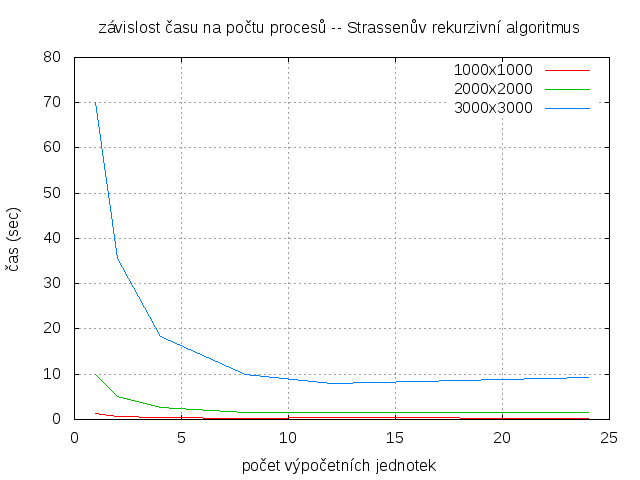
\includegraphics[width=\textwidth]{graph/strassen.png}
\caption{Strassenův rekurzivní algoritmus}
\label{data4}
\end{figure}

\pagebreak
\begin{figure}[h]
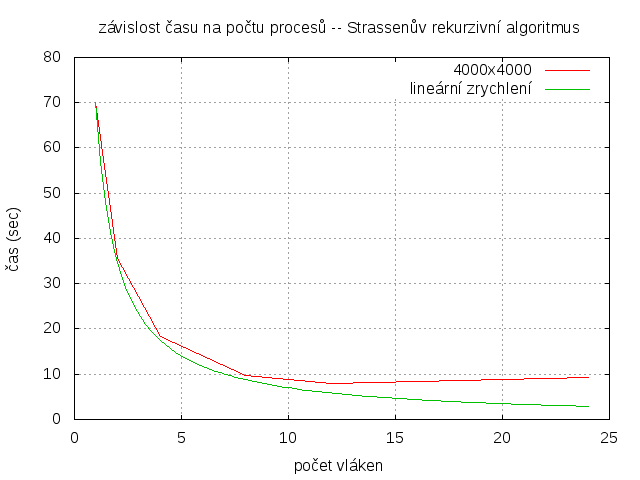
\includegraphics[width=\textwidth]{graph/strassen-4000.png}
\caption{Strassenův rekurzivní algoritmus pro matici 4000x4000}
\label{data4}
\end{figure}


\pagebreak
\begin{figure}[h]
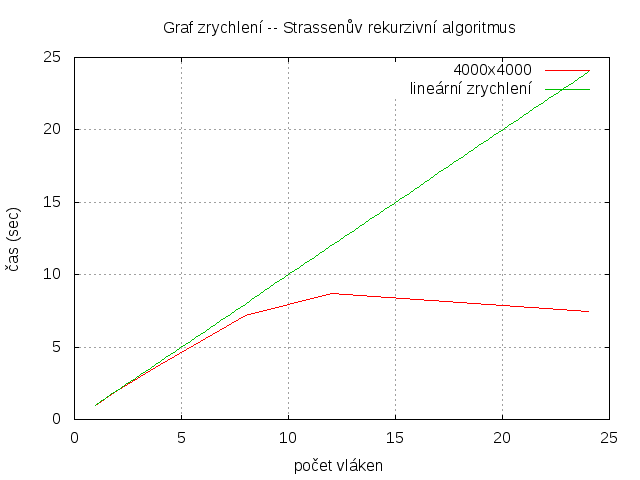
\includegraphics[width=\textwidth]{graph/strassen-acc.png}
\caption{Graf zrychlení -- Strassenův rekurzivní algoritmus pro matici 4000x4000}
\label{data4}
\end{figure}



\pagebreak
\subsubsection{Porovnání algoritmů}

\begin{figure}[h]
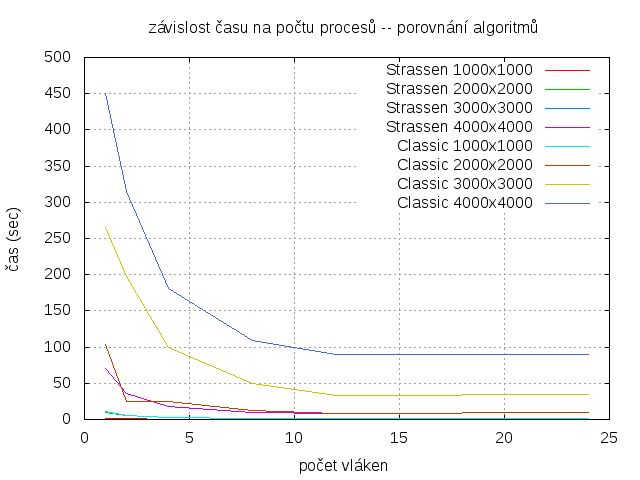
\includegraphics[width=\textwidth]{graph/classic-vs-strassen.png}
\caption{Porovnání obou algoritmů}
\label{data4}
\end{figure}

\pagebreak
\begin{figure}[h]
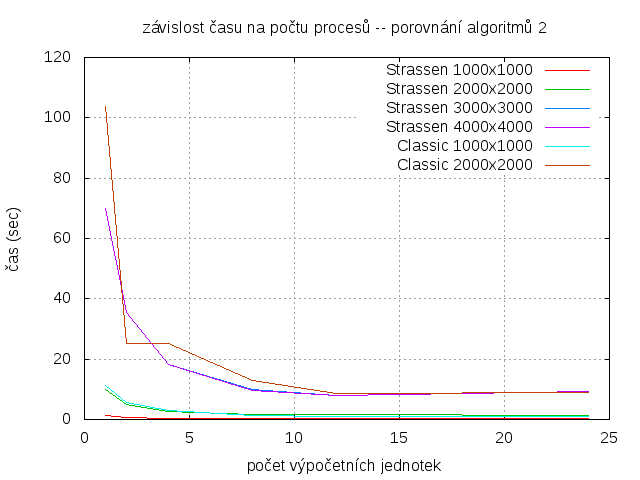
\includegraphics[width=\textwidth]{graph/classic-vs-strassen-2.png}
\caption{Porovnání obou algoritmů 2}
\label{data4}
\end{figure}

\pagebreak
\subsubsection{Porovnání plánování}

\begin{figure}[h]
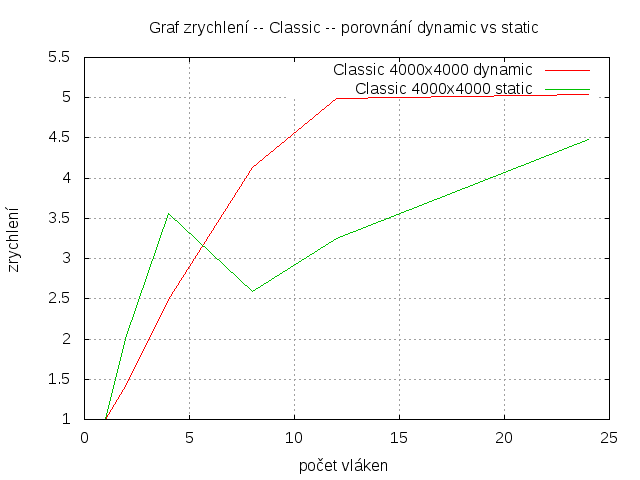
\includegraphics[width=\textwidth]{graph/classic-dynamic-vs-static.png}
\caption{Porovnání plánování dynamic vs static}
\label{data4}
\end{figure}

\pagebreak
\begin{figure}[h]
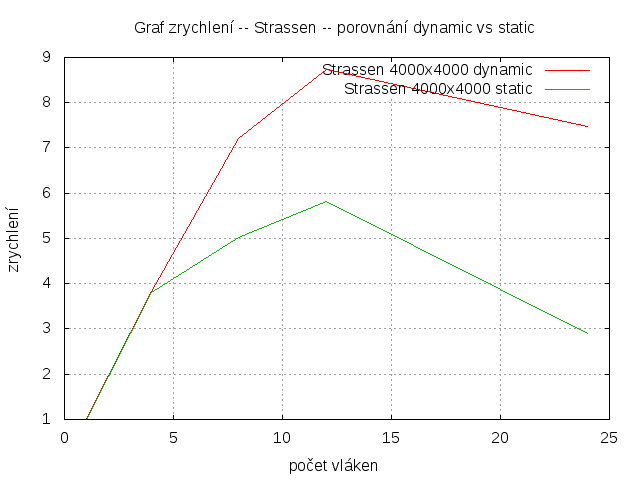
\includegraphics[width=\textwidth]{graph/strassen-dynamic-vs-static.png}
\caption{Porovnání plánování dynamic vs static}
\label{data4}
\end{figure}


\pagebreak
\subsection{Analýza a hodnocení vlastností dané implementace programu}

Byla naměřena relativně velká odchylka měření a podivná nekonzistence v~jednotlivých hodnotách. 
\bigskip

Zrychlení nad 12 jader není žádné. Předpokládám, že testovací server má 12 fyzických jader (a HyperThreading).

\subsubsection{Klasický multiplikační algoritmus}

Není dosaženo lineárního zrychlení.
\bigskip

Implementovaný algoritmus je časově i paměťové stabilní a předvídatelný.


\subsubsection{Strassenův rekurzivní algoritmus}

Je dosaženo téměř lineárního zrychlení, ale jen do 12ti výpočetních jader. Výsledky jsou k~mému překvapení lepší než u~klasického multiplikačního algoritmu.
\bigskip

Implementovaný algoritmus je paměťové velmi náročný a pro velmi, velmi velké vstupy by byl nepoužitelný. Mnoho času zabere režie s~pamětí a mnoho volání.
\bigskip

Nalezené řešení implementovaného algoritmu obsahuje chybu, která způsobuje drobné odchylky od reality. Chyba je stálá a není závislá na velikosti vstupu, času či míře paralelizace.

\subsubsection{Dynamické vs statické plánování}


Pro klasický multiplikační algoritmus je průběh zrychlení pro dynamické i statické plánování zcela odlišný. Statické plánování zde dosahuje menšího zrychlení, přestože zrychlení roste pro větší množství vláken než u dynamického plánování. \\


Pro Strassenův rekurzivní algoritmus je průběh zrychlení pro dynamické i statické plánování stejný, avšak dynamické plánování dosahuje většího zrychlení.


%****************************************
%****************************************
%
%				CUDA
%****************************************
%****************************************



\section{CUDA}
\subsection{Popis případných úprav algoritmu a jeho implementace}

Základ celého programu zůstal téměř nezměněn. Přidal jsem soubor \textit{simt\_trivial.cu}, který obsahuje celou implementaci (včetně měření) klasického multiplikačního algoritmu pomocí CUDA technologie. \\

Vstupní a výstupní matice jsou v C reprezentovány pomocí 2D pole. Při kopírování matice z paměti procesoru do paměti grafické karty (a naopak) proběhne transformace matice na 1D pole. \\

Všechny výpočty jsou v celočíselné.


\subsection{Popis optimalizací}

Snaha o saturaci každého bloku $1024$ vlákny, tedy využití všech $32$ warpů. \\

V implementaci jsem nepoužil \textit{loop unrolling}\footnote{Rozbalení cyklů -- např. počet průchodů cyklu zmenšíme na polovinu a v každém průchodu uděláme dvě operace najednou. Zmenšíme tak režii samotného cyklu vzhledem k potřebnému výpočtu.}.


\subsection{Naměřené výsledky}

$N$ je velikosti vstupních matic.

\begin{center}
\begin{tabular}{ | c || c | c | c | c | }
\hline
N    &   čas	\\
\hline
\hline
1000    &   0.20681 	\\ \hline
2000    &   0.39094 	\\ \hline
3000    &   0.82996 	\\ \hline
4000    &   1.27902 	\\ \hline
5000    &   2.92957 	\\ \hline
6000    &   4.28045 	\\ \hline
7000    &   7.42563 	\\ \hline
8000    &   8.21492 	\\ \hline
\end{tabular}
\end{center}

\pagebreak
\begin{figure}[h]
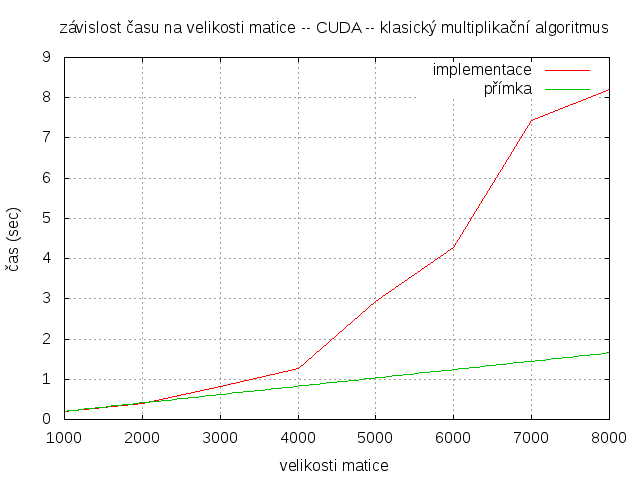
\includegraphics[width=\textwidth]{graph/cuda/cuda1.png}
\caption{Klasický multiplikativní algoritmus -- CUDA implementace}
\label{cuda1}
\end{figure}


\subsection{Analýza a hodnocení vlastností dané implementace programu}

Tato implementace algoritmu je násobně rychlejší než předchozí implementace na CPU. Zrychlení je velké, ale není lineární. \\

Algoritmus není efektivní ohledně přístupu do paměti. Zde by pomohlo například použití \textit{loop unrolling} nebo algoritmus přepracovat tak, aby uměl vhodně využít sdílenou pamět.


\section{Závěr}

\subsection{Porovnání výkonnosti všech tří verzí}




\end{document}
